\section{Solução Estrutural}

Antes de construir qualquer projeto estrutural é preciso realizar cálculos e simulações para descobrir se é viável as escolhas do projeto, além de saber se a estrutura planejada atende aos requisitos propostos.
\subsection{Cálculos estruturais}
\subsubsection{Resistência dos materiais}
Após análise dos possíveis materiais a ser usado como reforço principal, escolheu-se a cantoneira de aço comum como primeira opção. Contudo, precisa-se verificar através de cálculos se o material resistirá aos esforços aplicados.
\noindent \textbf{TENSÃO NORMAL}

A cantoneira tem como material principal o aço carbono simples, na qual é usinado com seção transversal com formato de L. As suas propriedades são as seguintes:
\begin{itemize}
	\item Área transversal: 96$mm^{2}$
	\item Tensão de escoamento: 350$Mpa$
\end{itemize}
A massa que estará sobre a estrutura está estimada para ser em torno de 10kg. Assim, o peso sobre a estrutura considerando uma gravidade de 9,8m/s$^{2}$ será de 98N. Aplicando a fórmula seguinte tem-se a tensão aplicada na estrutura.
\begin{equation}
\sigma = \frac{F}{A}
\end{equation}
onde F é a força aplicada e A é a área transversal da barra. Com isso, a tensão encontrada foi de 1,02MPa, distribuindo para as quatro barras de apoio fica 0,26MPa, onde a tensão aplicada é de mais de 1000 vezes menor do que a barra suporta. 
\noindent \textbf{FLEXÃO}
O material onde mais fica perceptível que ocorre flexão é a chapa de alumínio que servirá de fundo para a estufa. Assim, precisa-se calcular se não haverá ruptura. As propriedades do material são as seguintes:
\begin{itemize}
	\item Área transversal: 100$mm^{2}$
	\item Tensão de escoamento: 241$Mpa$
\end{itemize}
Em seguida calcula-se a tensão que sofrerá o alumínio considerando que o momento aplicado de acordo com a força é de 36,7N/m, o momento de inércia da área transversal é 6,46x$10^{-9} m^4$ e o c é $10^{-3}$m.
\begin{equation}
\sigma = \frac{Mc}{I}
\end{equation}
onde M é o momento aplicado no material, c é a distância entre o ponto neutro e a máxima distância da seção transversal e I é o momento de inércia. Com isso tem-se que a tensão aplicada é de 5,69MPa, na qual é 40 vezes menor do que a tensão de escoamento do alumínio.
\subsubsection{Vibrações naturais}

Existem duas formas de se calcular a frequência natural de um sistema, através de Métodos Matemáticos ou Métodos Experimentais. O método matemático consiste em cálculos analíticos ou modelos matemáticos computacionais (ex. Elementos Finitos), que são capazes de identificar as frequências naturais de uma estrutura. Fica evidente nesse caso, que a máquina não precisa ser construída para as frequências naturais serem identificadas, ou seja, se tratando de métodos matemáticos, apenas o projeto é suficiente para o cálculo das frequências naturais. Os métodos experimentais consistem em identificar as frequências naturais na própria peça física, ou seja, ela já deve estar construída. A ideia desse método é provocar uma vibração para que o sistema analisado entre em ressonância (frequência de operação = frequência natural) \cite{nobrega2014}.

No caso do nosso projeto, foi realizado o método matemático onde a análise modal, considerando todas as cargas e forças que atuarão no sistema foram analisadas através de simulações no software ANSYS. Com isso, para a determinação da frequência natural de Vibração da estrutura.  Logo, calculamos a Tensão Equivalente de Von Misses, como mostrado na seção de Simulações.

Um estudo da zona elástica do material da estrutura, no nosso caso a cantoneira, nos mostra as frequências naturais onde este material é capaz de suportar as vibrações que estejam dentro da vibração natural do material. Os dados para o aço são mostrados na figura \ref{fig:tabela_frequencia}.
\begin{figure}[H]
	\centering
	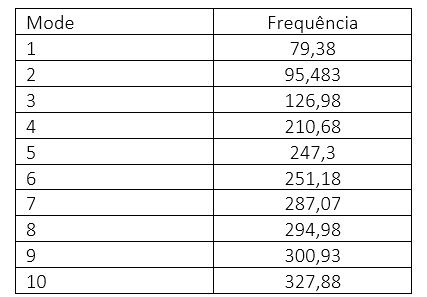
\includegraphics[width=10cm]{figuras/tabela_frequencia.png}
	\caption{Tabela de frequências naturais}
	\label{fig:tabela_frequencia}
\end{figure}

É importante ressaltar, que as mudanças realizadas na estrutura, através da utilização das chapas de MDF, Isopor e PVC, fazem com que a estrutura fique mais robusta, resistente e responde melhor as cargas com menores deformações. Analisando as tensões equivalentes de Von Misses com a tabela acima de vibração natural do aço, podemos observar que após a análise estática foi feita a análise dos modos de vibração na estrutura, com as frequências naturais de vibração da estrutura é possível modificar as frequências de rotação dos motores instalados na estufa com o intuito de não excitar a estrutura, mantendo essas frequências bem longes e evitando com que ocorra o processo de ressonância, podendo danificar a estrutura \cite{vencci2017}.
\subsection{Simulações}

Uma forma de conferir se os cálculos estão corretos, e em alguns casos até mesmo não precisar fazê-los, é utilizando simulações numéricas, que otimizam o tempo do engenheiro de forma simples e rápida.
\subsubsection{CATIA}

Como nem todos os componentes que farão parte final do projeto foram adquiridos antes das simulações, a equipe de estrutura não pode definir exatamente qual a massa que a estrutura suportaria dentro de si. Com isso, uma estimativa foi realizada para os cálculos. Após um brainstorm com integrantes de todas as áreas, a equipe chegou ao valor aproximado de 10kg, que engloba motores, sensores, válvulas, exaustores, plantário, tubos, canos, água, parafusos, roscas, reservatório e fiação.

Utilizou-se um fator de segurança 3 para qualquer tipo de inconveniente que possa ocorrer, ou seja, triplicamos a estimativa da massa esperada e encontramos o valor de 30kg. Arredondando o valor da aceleração da gravidade e utilizando a fórmula básica  encontramos uma força resultante axial sob a estrutura de 300 N. A equipe quis realizar diversos cenários de testes para checar o comportamento da estrutura mediante estes esforços e analisar as tensões de Von Mises e deslocamentos em diversas sessões do projeto a fim de buscar algum risco de ruptura. 

Como a massa estimada é muito baixa em relação ao que a estrutura pode suportar, as tensões e deslocamentos encontrados nas simulações conferem uma extrema segurança para o chassi levando em consideração os elevados limites de escoamento e ruptura que o material possui, dando assim confiança e liberdade para que a equipe continue os trabalhos sem problemas. As figuras dos CADs estão apresentadas da figura \ref{fig:catia1} até \ref{fig:catia11}.
\begin{figure}[H]
	\centering
	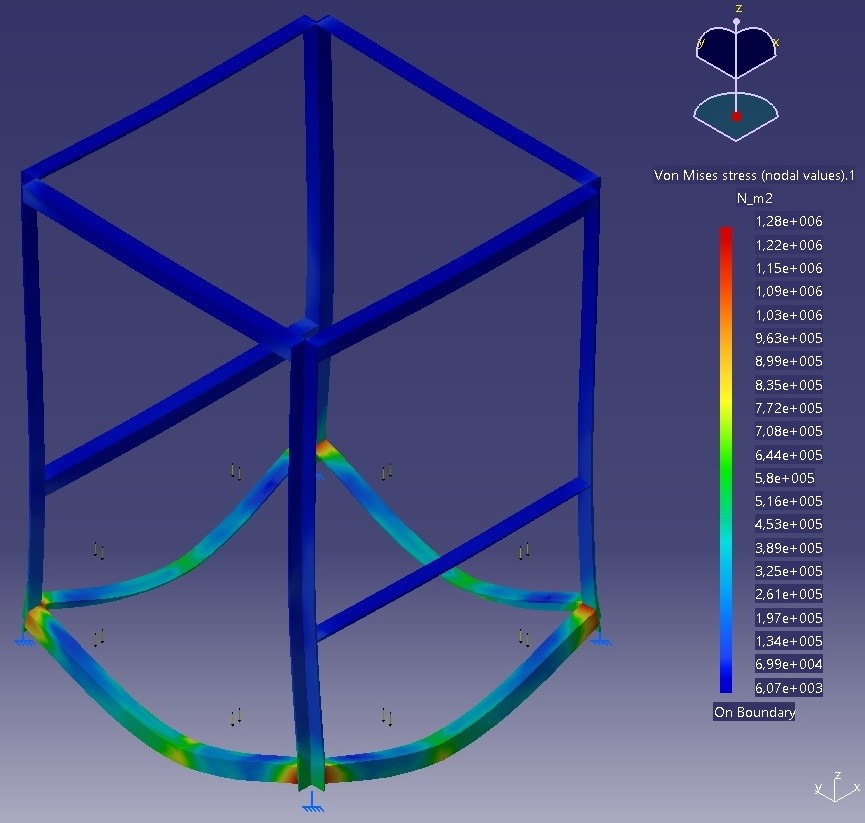
\includegraphics[width=10cm]{figuras/catia1.jpg}
	\caption{Análise de Tensão Von Mises do chassi aplicando 300 N nas 4 faces do assoalho}
	\label{fig:catia1}
\end{figure}
\begin{figure}[H]
	\centering
	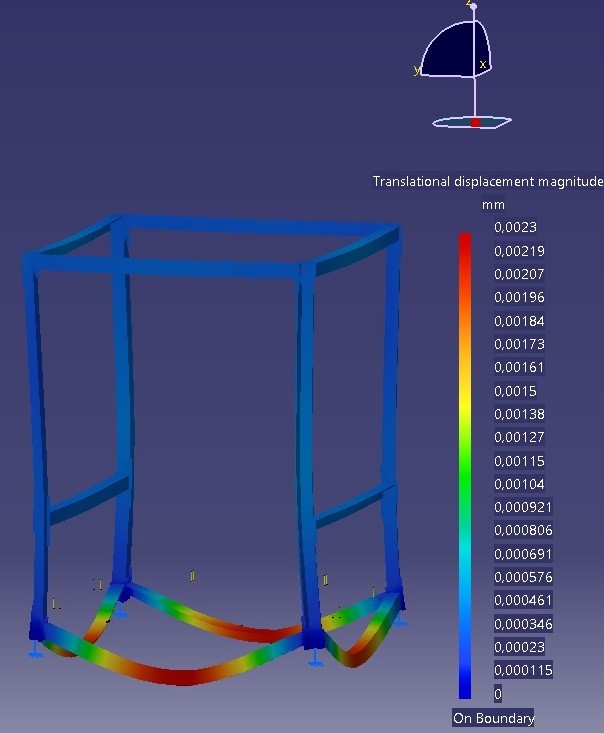
\includegraphics[width=10cm]{figuras/catia2.jpg}
	\caption{Análise da magnitude da deformação do chassi aplicando 300 N nas 4 faces do assoalho}
	\label{fig:catia2}
\end{figure}
\begin{figure}[H]
	\centering
	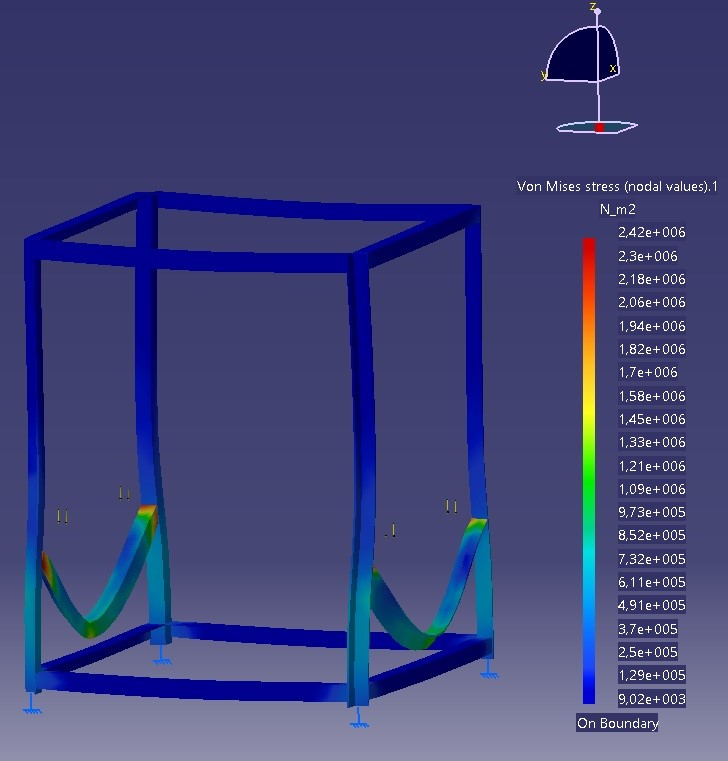
\includegraphics[width=10cm]{figuras/catia3.jpg}
	\caption{Análise de Tensão Von Mises do chassi aplicando 300 N nas barras de suporte laterais}
	\label{fig:catia3}
\end{figure}
\begin{figure}[H]
	\centering
	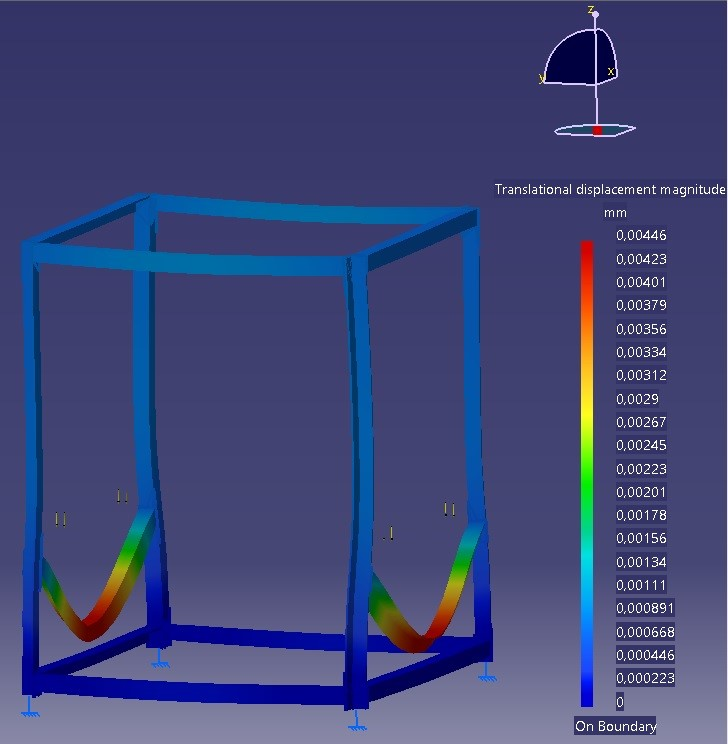
\includegraphics[width=10cm]{figuras/catia4.jpg}
	\caption{Análise de Tensão Von Mises do chassi aplicando 300 N nas barras de suporte laterais}
	\label{fig:catia4}
\end{figure}
\begin{figure}[H]
	\centering
	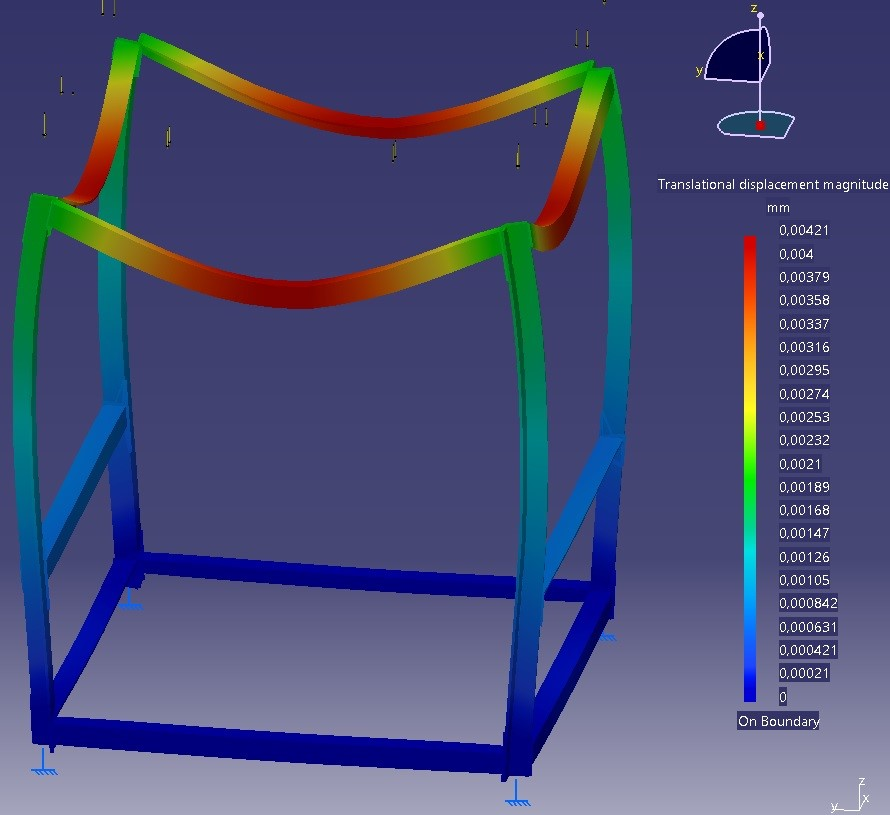
\includegraphics[width=10cm]{figuras/catia5.jpg}
	\caption{Análise da magnitude da deformação do chassi aplicando 300N nas 4 barras do teto}
	\label{fig:catia5}
\end{figure}
\begin{figure}[H]
	\centering
	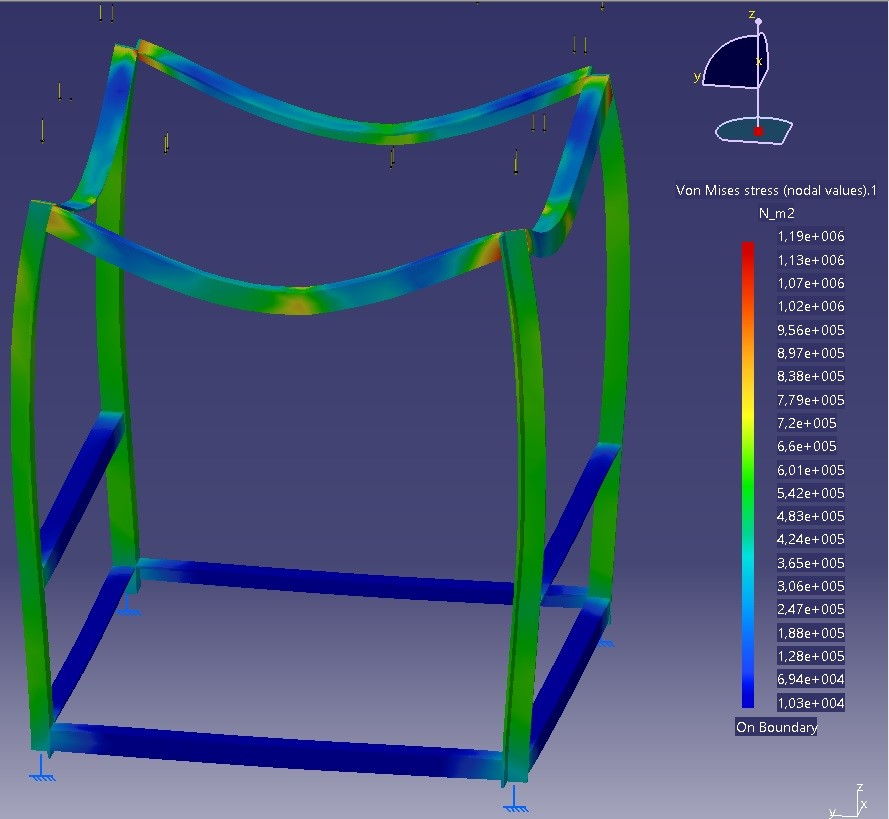
\includegraphics[width=10cm]{figuras/catia6.jpg}
	\caption{Análise da tensão Von Mises no chassi aplicando 300N nas 4 barras do teto}
	\label{fig:catia6}
\end{figure}
\begin{figure}[H]
	\centering
	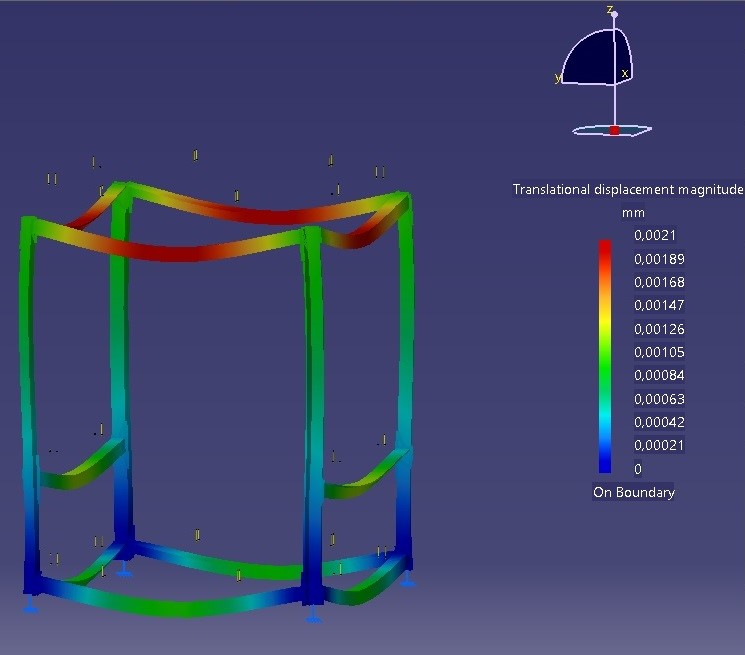
\includegraphics[width=10cm]{figuras/catia7.jpg}
	\caption{Análise da tensão Von Mises no chassi aplicando 300N em todas suas faces do plano XY}
	\label{fig:catia7}
\end{figure}
\begin{figure}[H]
	\centering
	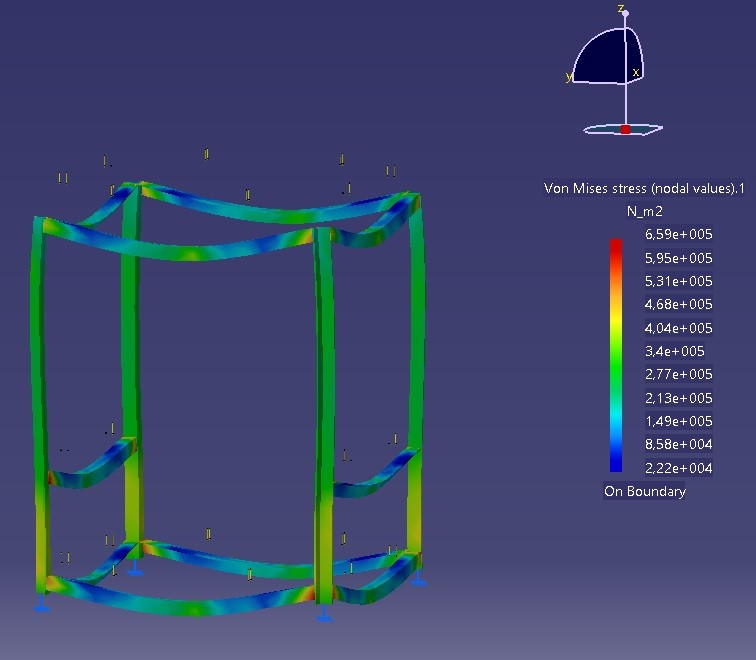
\includegraphics[width=10cm]{figuras/catia8.jpg}
	\caption{Análise da magnitude de deslocamento no chassi aplicando 300N em todas suas faces do plano XY}
	\label{fig:catia8}
\end{figure}
\subsubsection{ANSYS}

Para o bom crescimento das plantas é preciso que as temperaturas ambientes estejam adequadas. Sabe-se que a temperatura ideal deve estar entre 15 e 25$^{\circ}$C. Realizou-se uma simulação no software Ansys para analisar a viabilidade dos materiais. A figura \ref{fig:CAD_estufa} mostra o CAD da estufa no Ansys.
\begin{figure}[H]
	\centering
	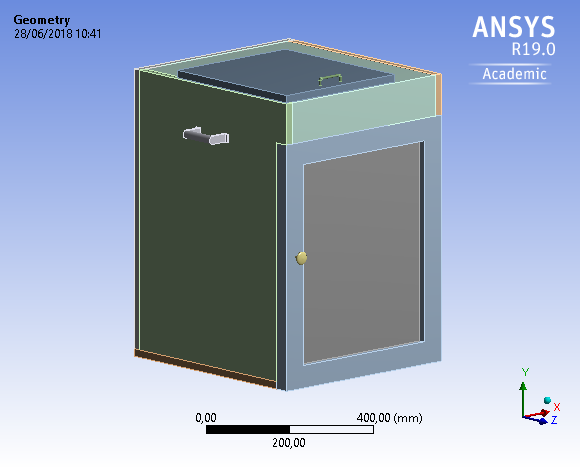
\includegraphics[width=10cm]{figuras/CAD_estufa.png}
	\caption{CAD da estufa completa}
	\label{fig:CAD_estufa}
\end{figure}

\subsubsubsection{Condições de Contorno}
\begin{itemize}
	\item Temperatura inicial externa de convecção: 30$^{\circ}$C
	\item Temperatura inicial da estufa: 22$^{\circ}$C
\end{itemize}
A transferência de calor se dará apenas por convecção do ar, onde o coeficiente de convecção é dado por , valor dado no Ansys para o ar.
\subsubsubsection{Resultado simulação}

Pela simulação nota-se que as escolhas dos isolantes foram certas, e cerca de 29 minutos depois a temperatura interna da estufa vai para 25$^{\circ}$C sem a atuação dos coolers de resfriamento. Com a atuação dos coolers essa temperatura é controlada para que nunca passe dos 25$^{\circ}$C. Pela simulação de transferência de calor na estufa percebe-se que a maior troca se dá pela porta de alumínio, como esperado por motivo de o alumínio ter a maior condutividade térmica, como mostram as figuras de \ref{fig:temperatura1} até \ref{fig:heatflux}. A figura \ref{fig:grafico_temperatura} apresenta a variação de temperatura máxima (vermelho), média (azul) e mínima (verde).
\begin{figure}[H]
	\centering
	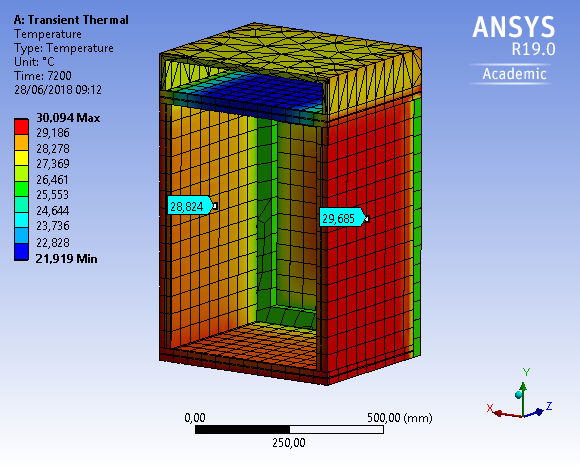
\includegraphics[width=10cm]{figuras/temperatura1.png}
	\caption{Temperatura final da estufa após uma hora de troca de calor sem refrigeração. Parte de trás com corte}
	\label{fig:temperatura1}
\end{figure}
\begin{figure}[H]
	\centering
	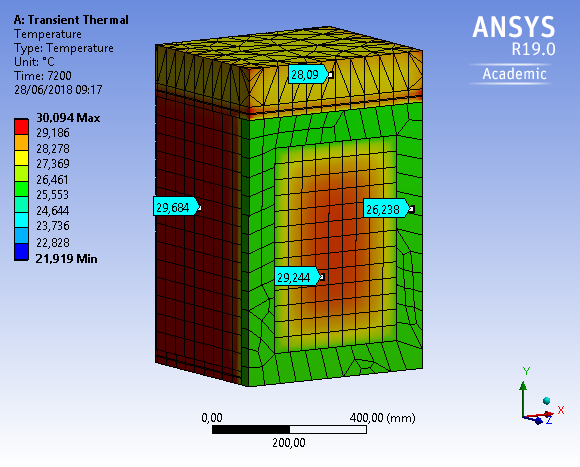
\includegraphics[width=10cm]{figuras/temperatura2.png}
	\caption{Temperatura final da estufa após uma hora de troca de calor. Parte da frente}
	\label{fig:temperatura2}
\end{figure}

\begin{figure}[H]
	\centering
	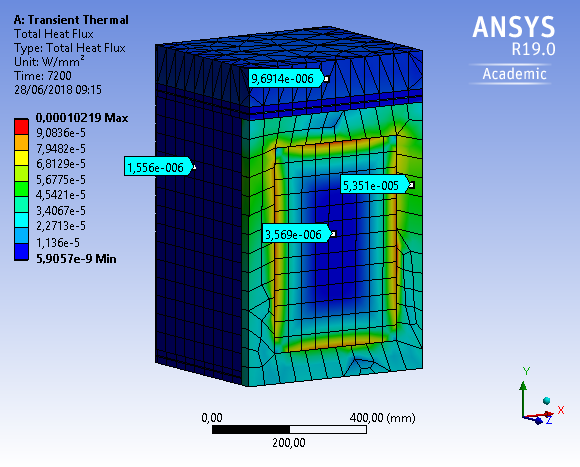
\includegraphics[width=10cm]{figuras/heatflux.png}
	\caption{Fluxo de calor na estufa após uma hora de troca de calor}
	\label{fig:heatflux}
\end{figure}
\begin{figure}[H]
	\centering
	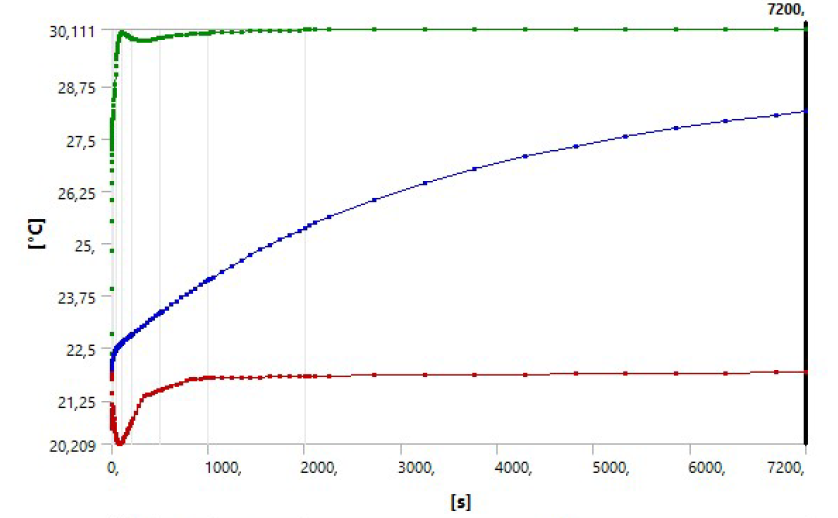
\includegraphics[width=10cm]{figuras/grafico_temperatura.PNG}
	\caption{Variação da temperatura na estufa ao longo de duas horas}
	\label{fig:grafico_temperatura}
\end{figure}